\bodychapter{EXAMPLES}
\label{examples}

In order to help explain the property mapping process, we present an introduction to the interface, followed by a few examples.

The interface (Figure~\ref{fig:interface}) has four main components.
The left side contains a list of all of the data dimensions loaded into the tool.
The green figures at the top of the screen are buttons for creating new primitives.
In Figure~\ref{fig:interface}, the circle on the right side with the lists of items is a prototype circle primitive.
The golden list on the left side of the circle is the input properties, and the blue list on the right side is the output data from the primitive.
The triangles above each property are scale handles.

Mousing over each property shows the current scale value, and if the property is mapped, highlights the data field that the property is connected to (in this case, area is connected to EmploymentRate).
The grayed out properties are not available because area is mapped, and through the internal geometric relationships that defines the radius and circumference of the circle.
Property mappings are accomplished by clicking on any blue data buttons, and then clicking on any gold property buttons.
Scaling of a mapped property is accomplished by clicking and dragging the triangular handle left or right.

The blue circles are the instances of the primitive that are being specified by the prototype circle.
Together they show the visualization that is produced by the mappings of the prototype.
To prevent occlusion of the visualization, the prototype can be moved around the canvas area by clicking and dragging.
The visualization itself can also be moved around the canvas to help keep all instances on screen (in the case of extremely high or low values).
Dragging the visualization will move all instances of all primitives as a group, in order to keep the data defined relationships intact.
(To try the interface yourself, you may visit~\url{http://visualizationprimitives.net}.)

\begin{figure*}[t]
\centering
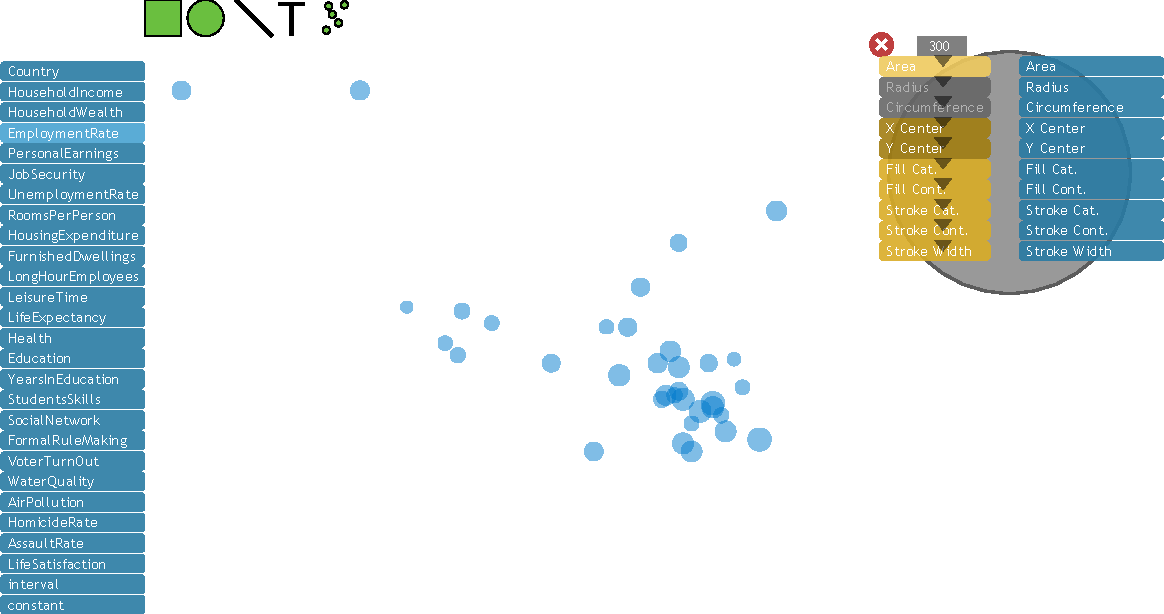
\includegraphics[width=\textwidth]{images/interface.pdf}
\caption{The interface for the current implementation of Visualization Primitives.}
\label{fig:interface}
\end{figure*}

The following examples show how to construct existing familiar visualization types.
Some of them show interesting concepts that are highlighted when producing visualizations from a primitives based approach.
Along with the description of how to construct them, we present versions of each visualization created with our current implementation of visualization primitives.

\bodysection{Bar Chart}
\label{barChart}

Bar charts are created with a rectangle primitive.
In a bar chart, the rectangle only has one data driven visual property, height.
The rectangle's other properties are all derived from administrative data.
Horizontal position is tied to a sequence, while other properties are all tied to a constant.

To create a stacked bar chart, a new rectangle primitive can be connected to the existing rectangle primitive (Figure~\ref{fig:stackedBar}).
To make the connection, the top side of the original rectangle is used as the input for the bottom side of the new rectangle.
They share the same horizontal positions and widths, and the height comes from a separate data source.
Users design not only the prototype primitive, but also the relationships between the prototype primitives.

To create a grouped bar chart, the data assignments are similar (Figure~\ref{fig:groupedBar}).
The two rectangles share the same bottom side position, and the same width, and the height of the new rectangle still comes from external data.
But now the left side of the new rectangle is connected to the right side of the original rectangle.

\begin{figure*}[t]
\centering
\hfill
\subfigure[Stacked Bar Chart]{
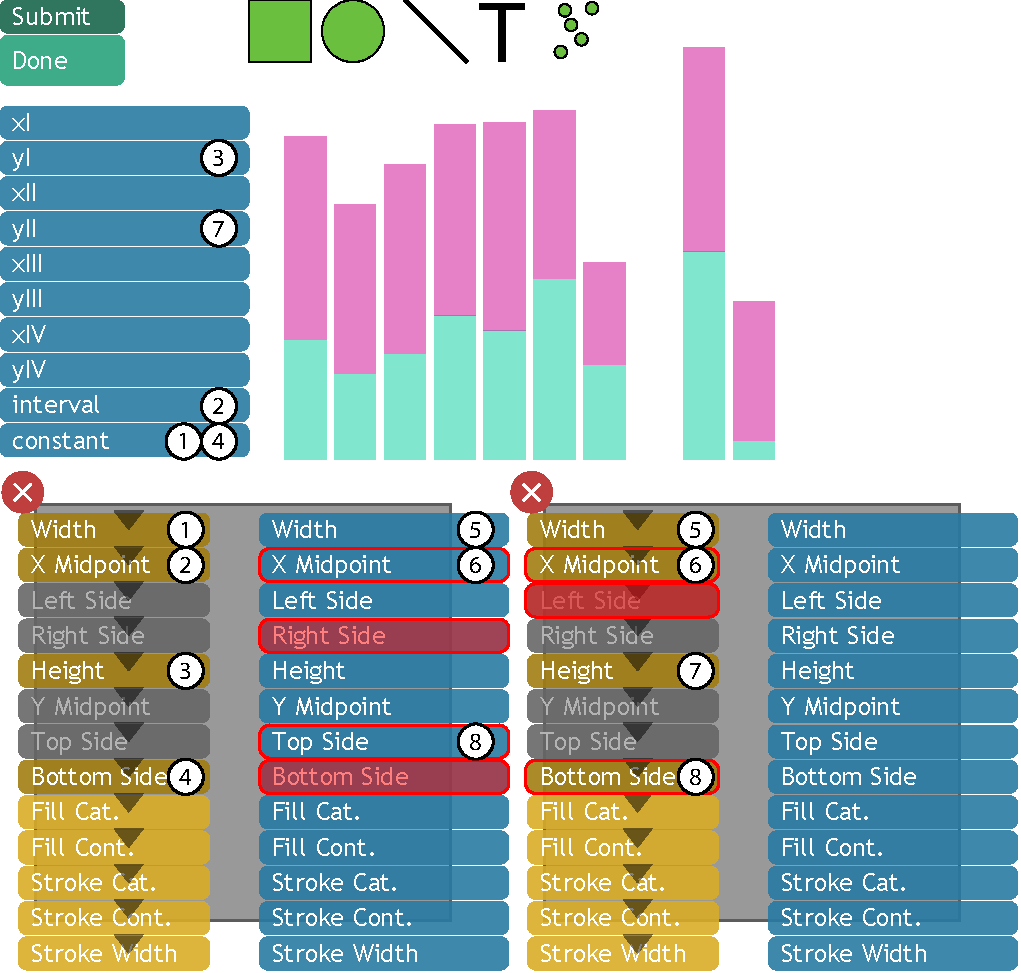
\includegraphics[width=.4\columnwidth]{images/stackedBar.pdf}
\label{fig:stackedBar}
}
\hfill
\subfigure[Grouped Bar Chart]{
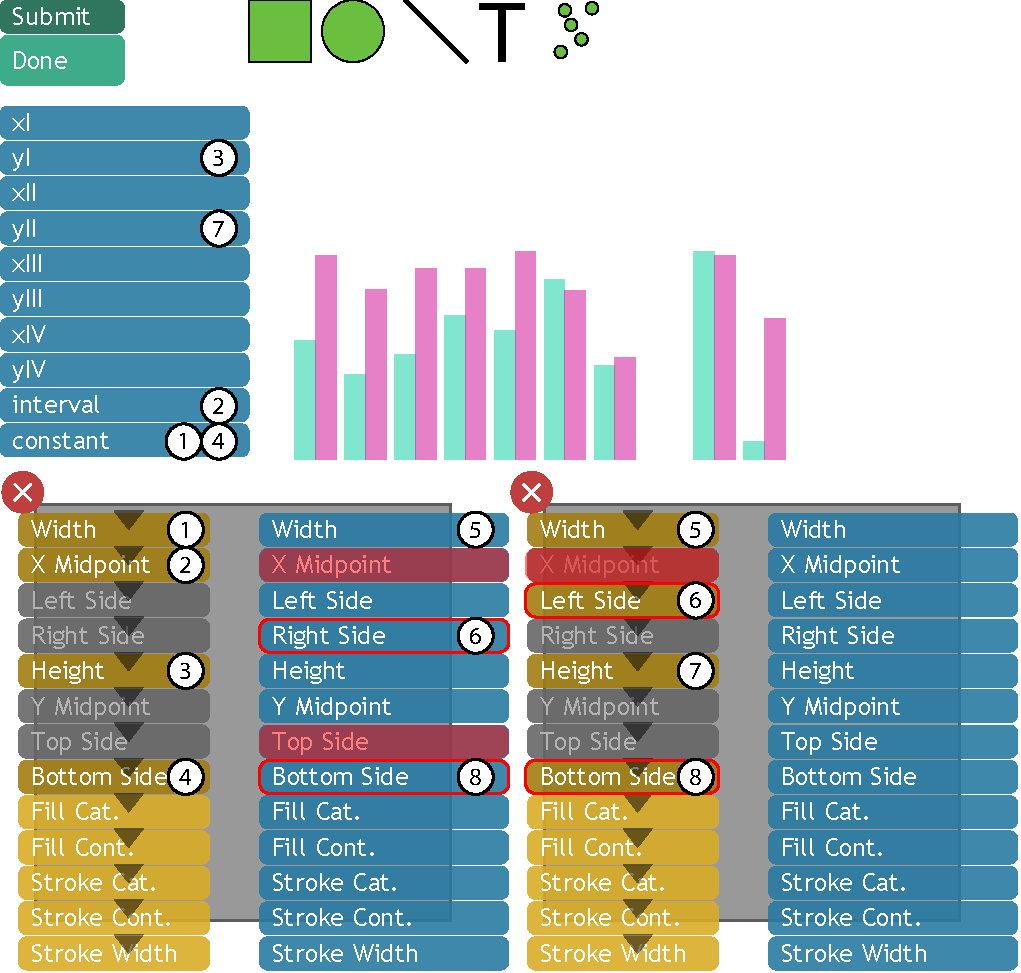
\includegraphics[width=.4\columnwidth]{images/groupedBar.pdf}
\label{fig:groupedBar}
}
\caption{A stacked bar chart and grouped bar chart in our implementation.
The data in both is from Anscombe's Quartet~\cite{Anscombe1973}.
Stacked bars (a) and grouped bars (b) differ only in the mapping of their sides.
The numbers are added to indicate mappings, in the interface mouseover provides this information.
The red highlights indicate the differences in the mappings between the two charts.
}
\label{fig:barCharts}
\end{figure*}

\bodysection{Scatterplot}
\label{scatterplot}

A standard scatterplot showing only one category is easily created with a circle primitive.
Horizontal and vertical position of the shape are the two data driven properties.
The other properties are all administrative.
For some datasets, a scatterplot can represent additional values with the color or size properties.

Scatterplots are very simple to create with our implementation (Figure~\ref{fig:scatterplot}).
In this example a circle has been used, but any primitive in our implementation has the horizontal and vertical position properties that are necessary.
Connecting a categorical value (in this example, number of cylinders) to the fill color property, maps the value to a member of a categorical color scale.

Other primitives designed for scatterplots could provide a categorical visual variable of shape.
This variable would provide access to a set of shapes for representing categorical data.

\begin{figure*}[t]
\centering
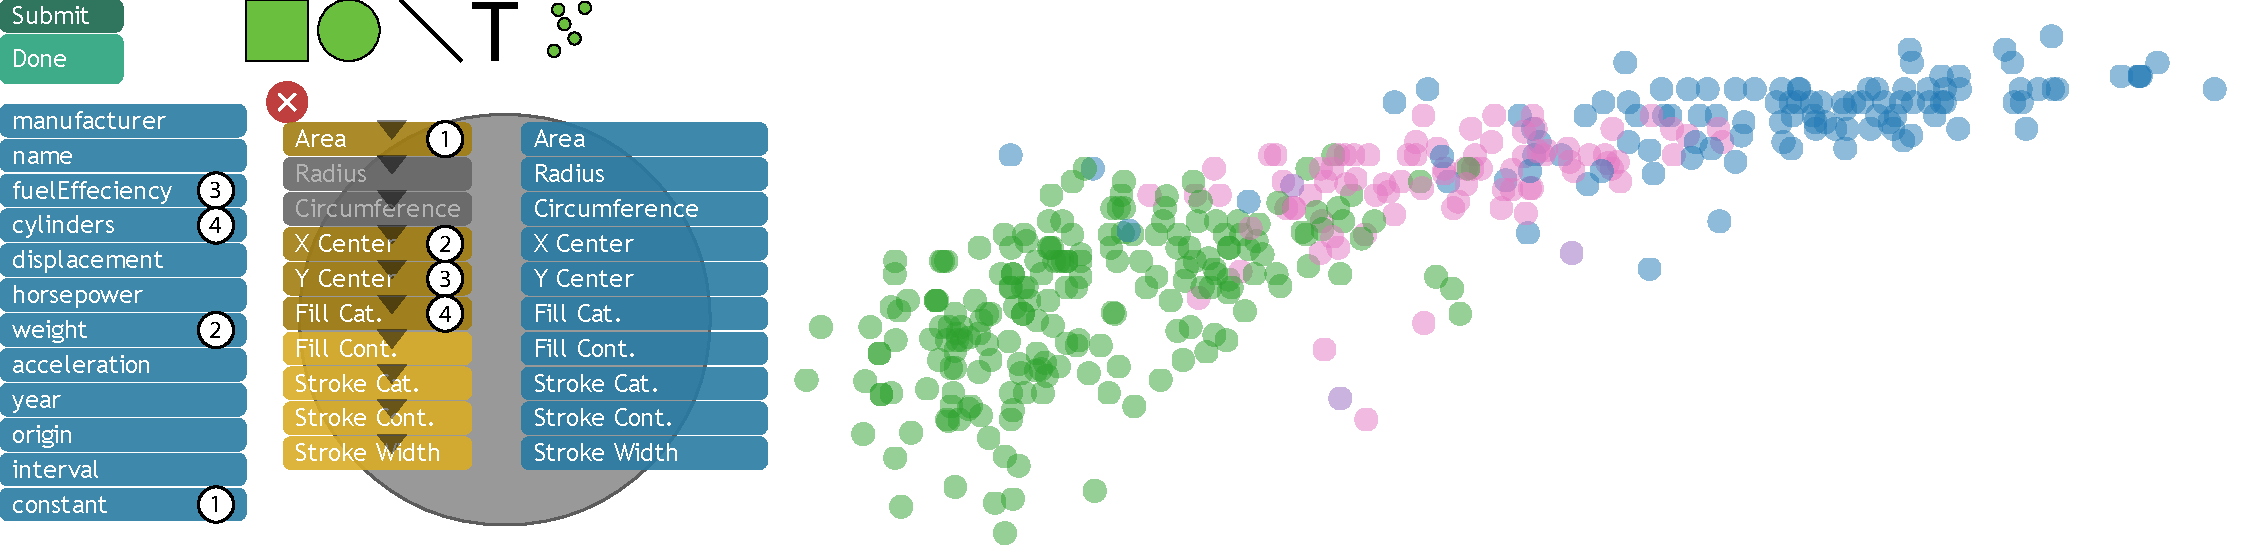
\includegraphics[width=\textwidth]{images/scatterplot.pdf}
\caption{A scatterplot in our implementation using the UCI cars dataset.
Miles per gallon is attached to vertical position, weight is attached to horizontal position.
Number of cylinders is connected to color.
The numbers are added to indicate mappings, in the interface mouseover provides this information.
}
\label{fig:scatterplot}
\end{figure*}

\bodysection{Line Chart}
\label{lineChart}

Line charts are a unique case.
They break the information visualization model slightly by indicating continuity within a data dimension.
This special case requires special treatment in the visualization primitives model.

Line charts need to have the iteration of some of their data to be offset by one.
This makes the two endpoints of the line instances refer to different items in the data, and creates the visual continuity between each data item.
Without this connection, a line chart would simply be a series of points.

There are a number of ways this can be accomplished in the visualization primitives model.
Since a line chart without connections decomposes into points, we opted to make the points primitive allow connections between each point instance.
This allows the line primitive to keep an angular property for creating texture effects.

In a line chart, just like a bar chart, the primitive has one essential visual property.
The remaining properties are all administrative, and only serve to create the layout.

For point primitives in our implementation, the connectedness of the points is also a property.
This allows connections to be driven by data, although in a line chart, connections are mapped to a constant value to turn them on for all instances (Figure~\ref{fig:lineChart}).
When the point primitive draws its instances in the visualization view, it grabs the position for the connection's other end from its previous sibling in the data.
In our current implementation, this uses the existing order of data, however future implementations will include ways to sort data by any of the data dimensions.

\begin{figure*}[t]
   \centering
   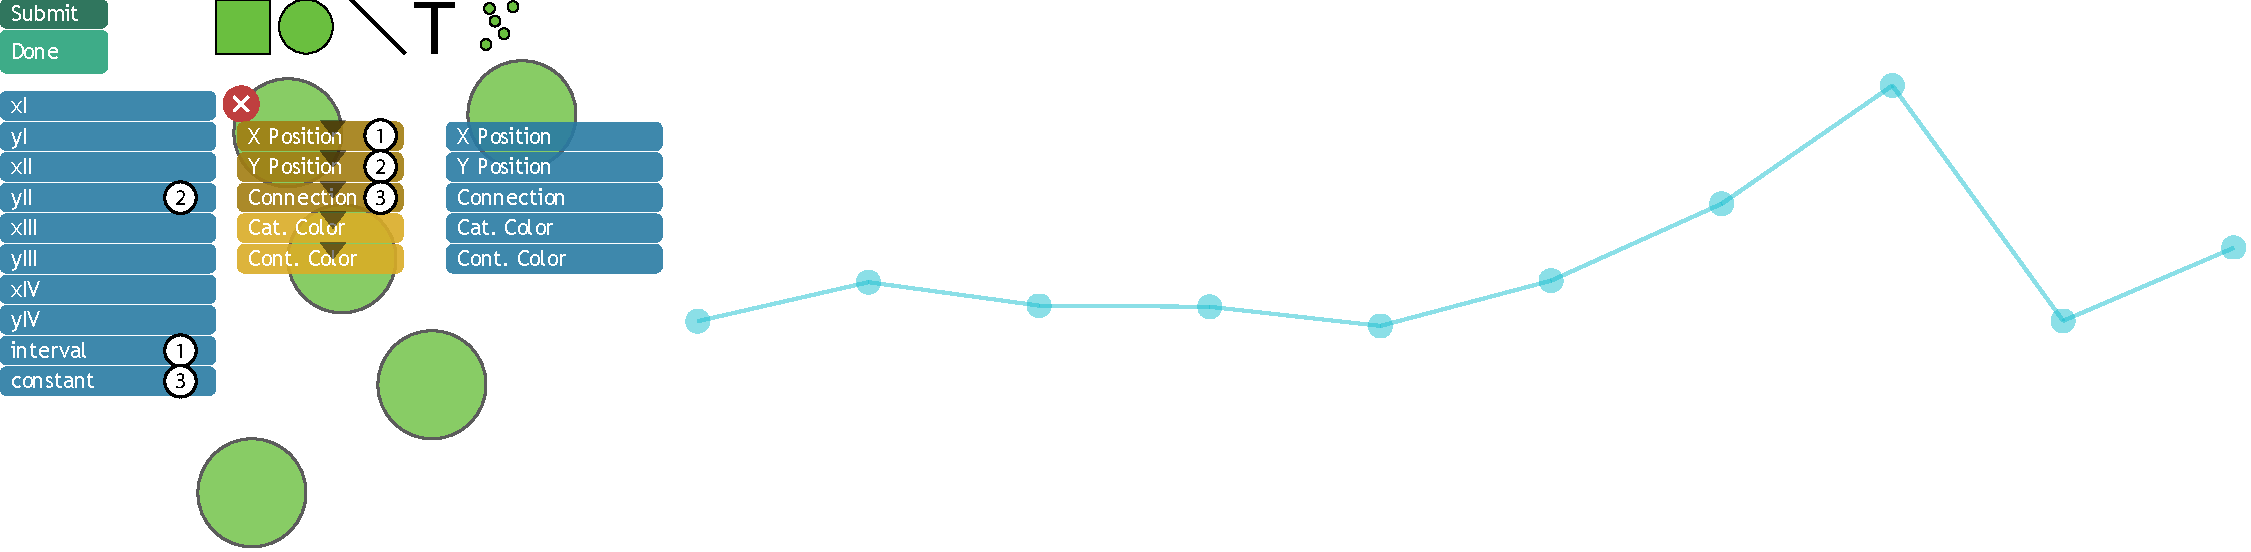
\includegraphics[width=\textwidth]{images/lineChart}
   \caption{
   A line chart in our implementation is created by turning on a connection between points.
   The numbers are added to indicate mappings, in the interface mouseover provides this information.
}
   \label{fig:lineChart}
\end{figure*}

\bodysection{Heat Maps}
\label{heatMap}

Periodic data is often represented in heat map grids where color is tied to data, while time data build the grid (Figure~\ref{fig:heatMap}).
With the right breakdown of time in the data, this is also a simple visualization to create with visualization primitives.
Our example uses Typical Meteorological Year 3 data for Charlotte, NC~\cite{wilcox2008users}.
One data field indicating day of the year is mapped to the vertical position, while horizontal position comes from the hour of the day.
The width and height of the primitive instances comes from a constant value.
The color scale is tied to the dry bulb temperature.
\begin{figure}[t]
   \centering
   \includegraphics[width=.5\columnwidth]{images/heatMap}
   \caption{
   A heat map of temperature using TMY3 data~\cite{wilcox2008users}.
   The numbers are added to indicate mappings, in the interface mouseover provides this information.
}
   \label{fig:heatMap}
\end{figure}

\bodysection{Waterfall Chart}
\label{waterfallChart}

Related to the gantt chart, a less well known chart is the Waterfall Chart (Figure~\ref{fig:presidents}).
This chart type is useful for seeing trends in timeline data.
In our implementation, the chart is created using three primitives showing data on United States Presidents.
One rectangle primitive shows the lifespan of the presidents.
The left side is mapped to birthday, the right side is mapped to the day of their death (or the current date).
The height is assigned a constant value, and the vertical position is a sequence.
Another rectangle primitive displays the presidents' time in office.
The left side is mapped to their inauguration, while the right is mapped to the end of their term.
The height and vertical position come from the respective outputs on the other rectangle primitive.
A text primitive labels the names of each president.
The text string is mapped to the names field.
The left side comes from the right side of the lifespan rectangle, while the vertical position and height are mapped to the respective properties of the lifespan rectangle.
\begin{figure*}[t]
   \centering
   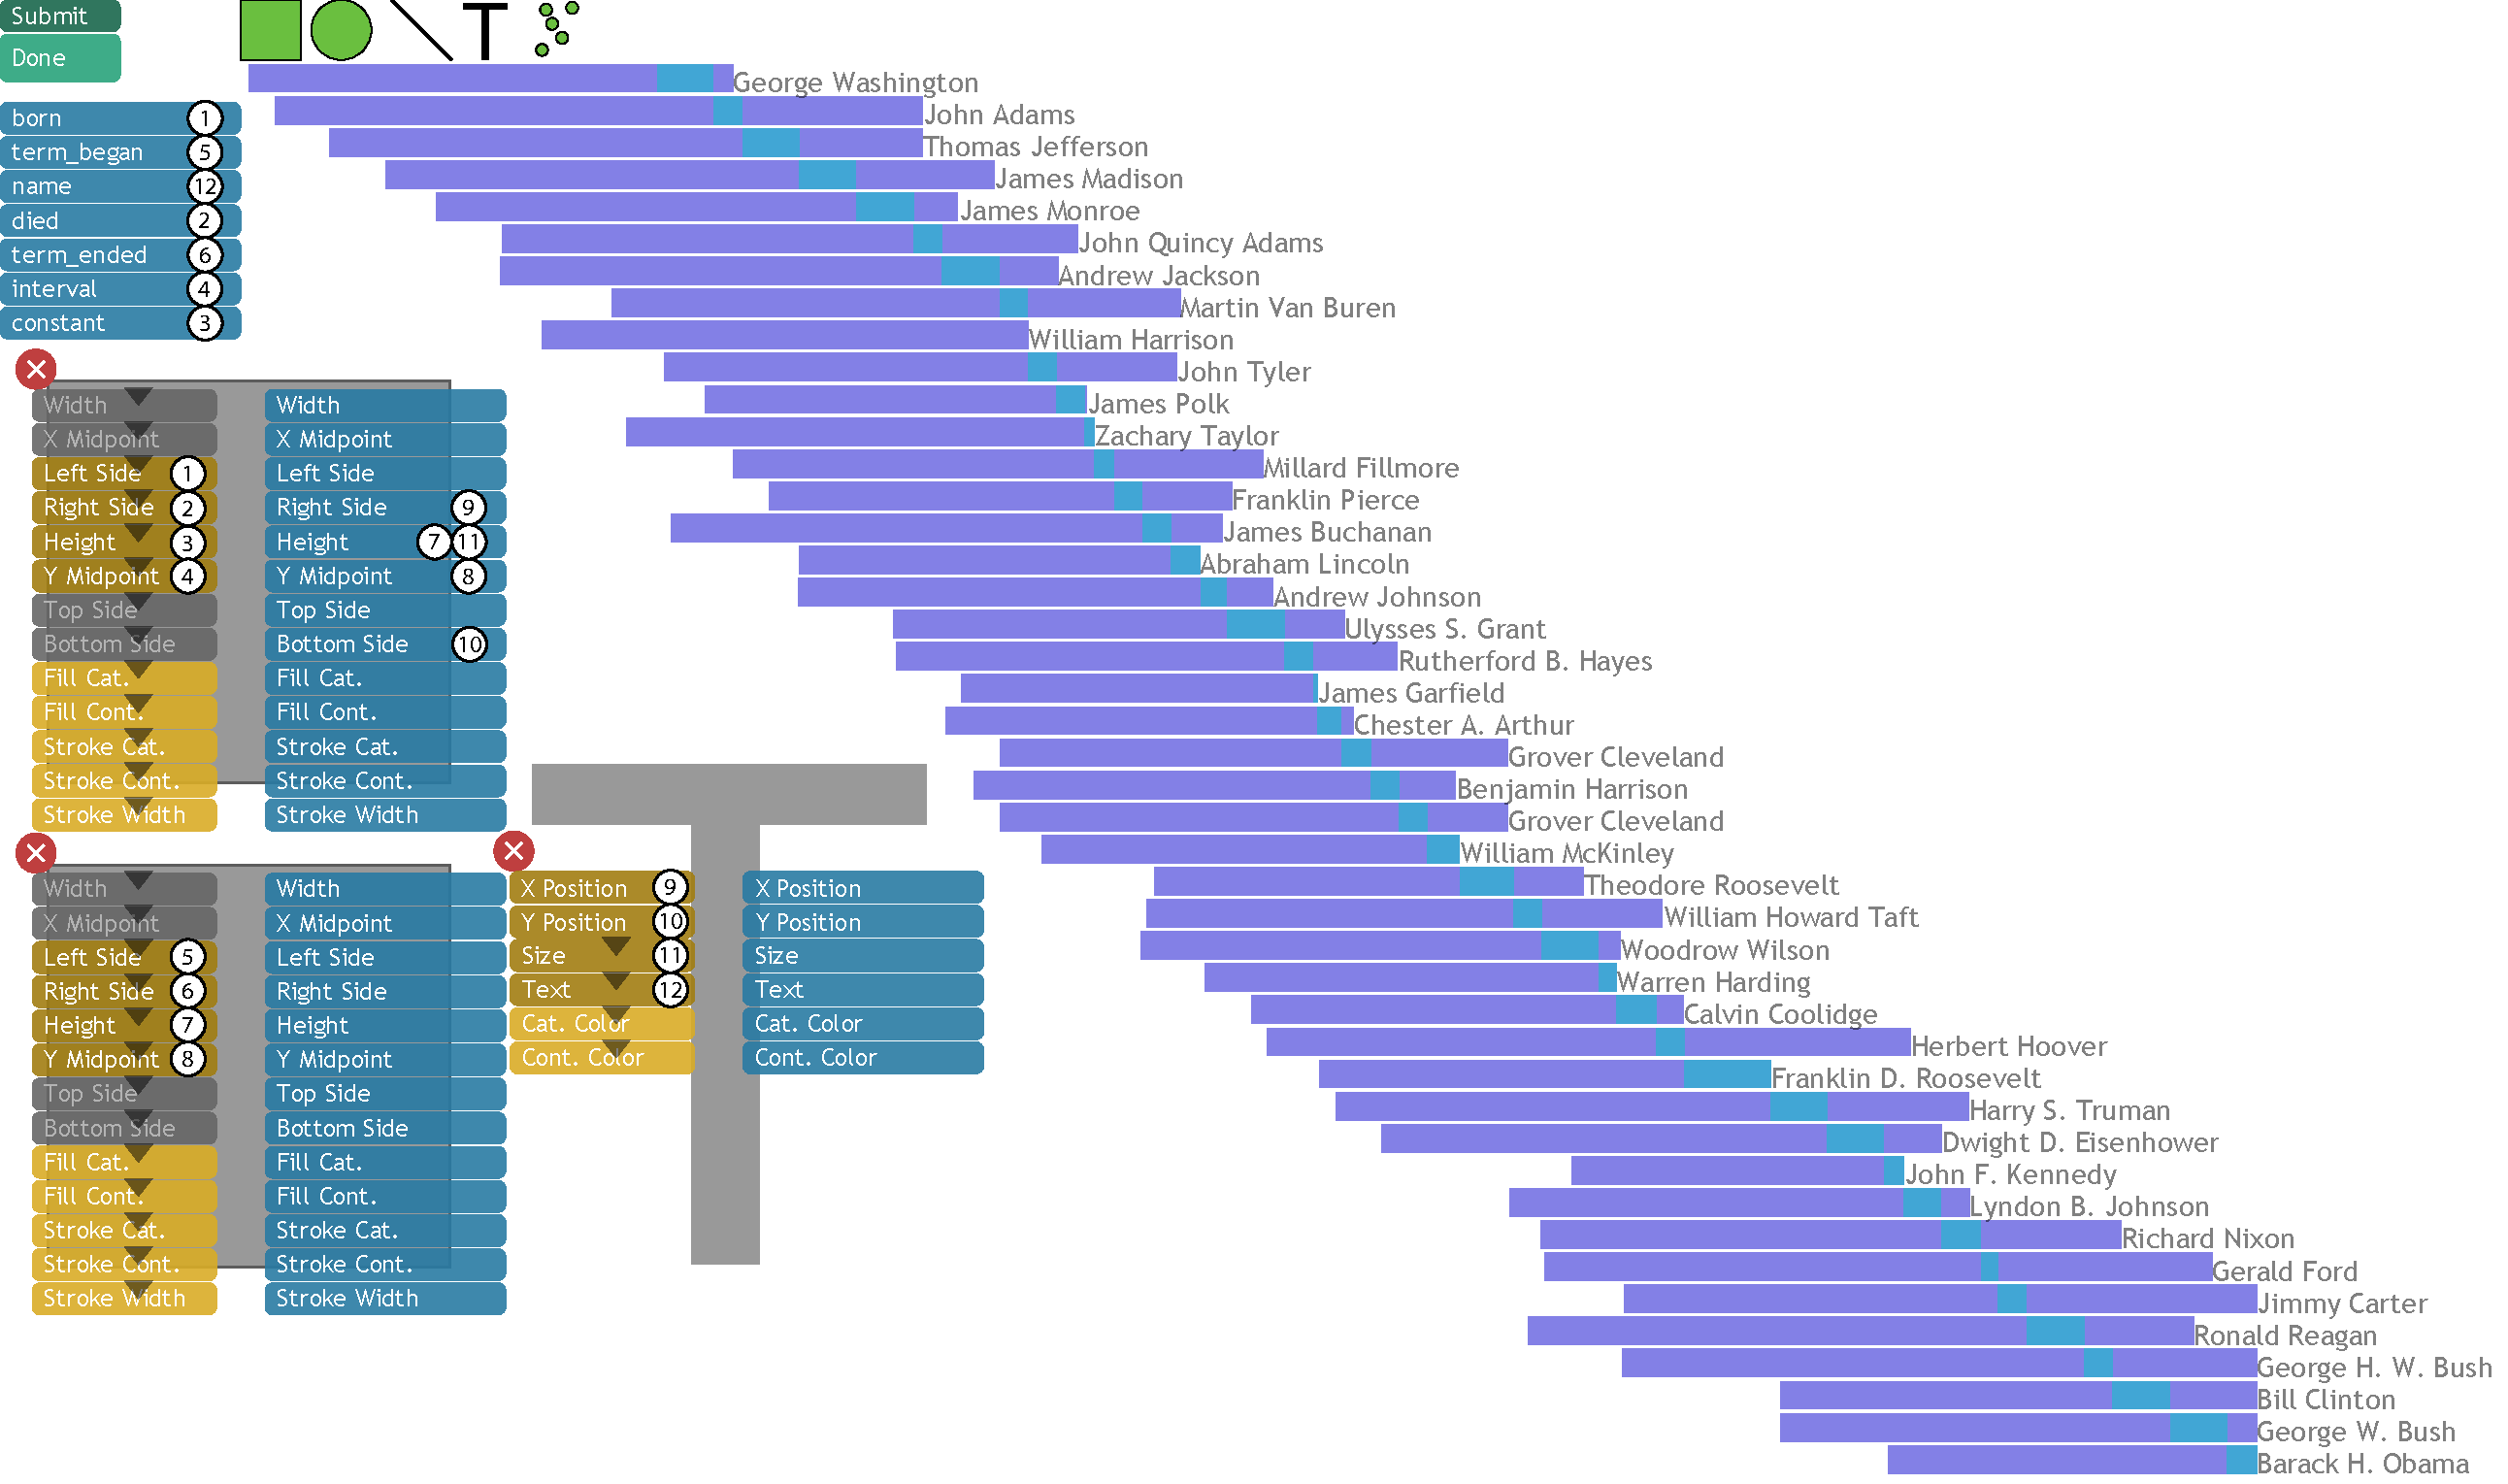
\includegraphics[width=\textwidth]{images/presidents}
   \caption{
   A waterfall chart showing the lifespans and terms of the presidents of the United States.
   The numbers are added to indicate mappings, in the interface mouseover provides this information.
}
   \label{fig:presidents}
\end{figure*}

\bodysection{Glyphs}
\label{glyphs}

Glyphs~\cite{Horn1998} are often used to create small multiples for comparison.
An example of this technique implemented in our system can be seen in Figure~\ref{fig:cars}.
The visualization is built using the cars dataset.
This visualization is not an existing chart type, but is an example of a novel visualization created using visualization primitives.
Four primitives make up each glyph, with each primitive representing a dimension of the data.
Horsepower is the width of the blue rectangles, fuel efficiency is the width of the green rectangles.
The yellow-green ``wheels'' show weight, while the blue ``wheels'' show acceleration.

\begin{figure}[t]
\centering
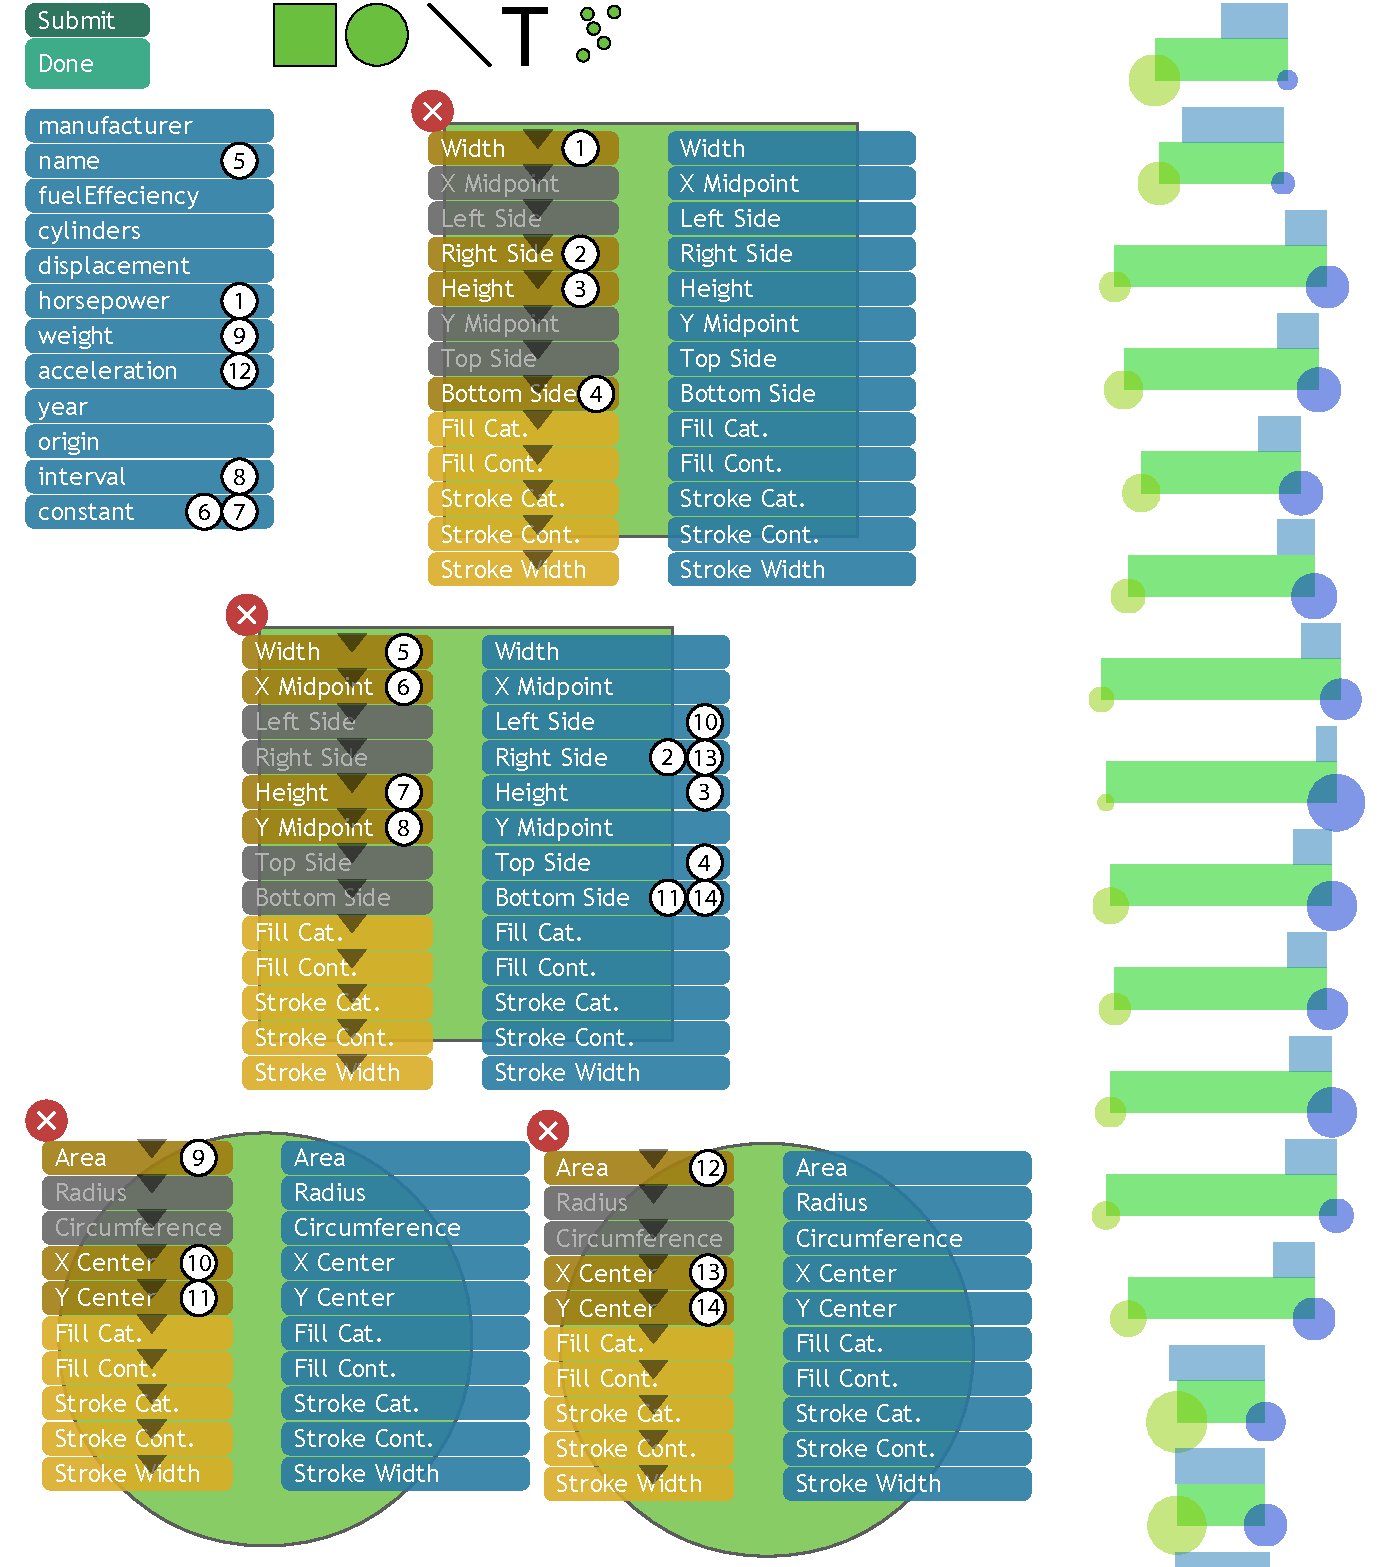
\includegraphics[width=.5\columnwidth]{images/cars.pdf}
\caption{
A glyph technique in our implementation using the cars dataset. The technique is similar to the one used in VIE-VISU~\cite{Horn1998}.
The numbers are added to indicate mappings, in the interface mouseover provides this information.
}
\label{fig:cars}
\end{figure}